\documentclass[11pt]{article}
\usepackage[utf8]{inputenc}
\usepackage[ngerman]{babel} % change accordingly

\usepackage{amsmath,amsthm,amssymb,amsfonts}

\usepackage{graphicx}
\graphicspath{{abb/2-vektoren/}}
\usepackage{float}
\usepackage{tikz}

\usepackage{fancyhdr} % for headers and footers
\usepackage{geometry}
\usepackage{listings}

\usepackage{hyperref}
\hypersetup{
    linkcolor=blue,     
    urlcolor=cyan,
}

\geometry{
    a4paper, 
    left=20mm,
    right=20mm,
    top=30mm,
    bottom=30mm,
}

\newcommand{\N}{\mathbb{N}}
\newcommand{\Z}{\mathbb{Z}}
\newcommand{\R}{\mathbb{R}}
\newcommand{\Q}{\mathbb{Q}}
\newcommand{\C}{\mathbb{C}}

\newcommand{\e}{\mathrm{e}}

\newcommand{\abs}[1]{\left \lvert #1 \right \rvert}
\newcommand{\floor}[1]{\left \lfloor #1 \right \rfloor}
\newcommand{\ceil}[1]{\left \lceil #1 \right \rceil}

\newcommand{\liminftyn}{\lim\limits_{n \rightarrow \infty}}

\newcount\colveccount
\newcommand*\colvec[1]{
        \global\colveccount#1
        \begin{pmatrix}
        \colvecnext
}
\def\colvecnext#1{
        #1
        \global\advance\colveccount-1
        \ifnum\colveccount>0
                \\
                \expandafter\colvecnext
        \else
                \end{pmatrix}
        \fi
}

\title{Vektoren}
\author{Anna Bodnar \& Emil Staikov}
\date{5. März 2021}

\begin{document}
\maketitle
Bis jetzt haben wir nur Bewegungen auf Geraden betrachtet, und eine Beschreibung der Bewegungsparameter (Weg, Geschwindigkeit, ...) durch normale Zahlen (Skalare) hat ausgereicht. Wenn wir aber nun eine Bewegung wie einen Wurf betrachten, ändert sich sowohl Richtung als auch Größe der Geschwindigkeit, und der absolute Abstand vom Abwerfenden (Betrag des Abstands) reicht nicht mehr aus, um die Lage des geworfenen Gegenstandes eindeutig zu beschreiben. Um unsere Größen in mehreren Raumrichtungen zu beschreiben, führen wir das Konzept von Vektoren ein. 

\section{Definition}
Eine vektorielle Größe hat Betrag und Richtung, im Gegensatz zum Skalar, welcher durch seinen Betrag vollständig bestimmt ist. Einen Vektor stellen wir durch seine Komponenten dar, das sind die voneinander unabhängigen Teile des Vektors entlang bestimmter Achsen. Unabhängig heißt hier, dass die Änderung einer Komponente nicht zu einer Änderung der anderen Komponenten führt. Vektoren sind für beliebig viele Raumrichtungen (bzw. Dimensionen) definiert, wir betrachten hier jedoch nur den zweidimensionalen Fall. Allgemein ist ein Vektor durch seine Komponenten vollständig bestimmt: 
$$\vec{a} = \colvec{2}{a_x}{a_y} = a_x\hat{e_x} + a_y\hat{e_y}$$
Dabei ist $a_x$ die Komponente (bzw. "Länge") in x-Richtung und $a_x$ die Komponente in y-Richtung, $\hat{e_x}$ und $\hat{e_y}$ sind die sogenannten Einheitsvektoren in die jeweiligen Richtungen. Sie zeigen in x- bzw. y-Richtung und haben die Länge 1. Einen Vektor verdeutlichen wir durch den Pfeil über ihm, eine Ausnahme bilden eben die Einheitsvektoren, diese haben ein Dach über sich. Grafisch: 
\begin{figure}[H]
    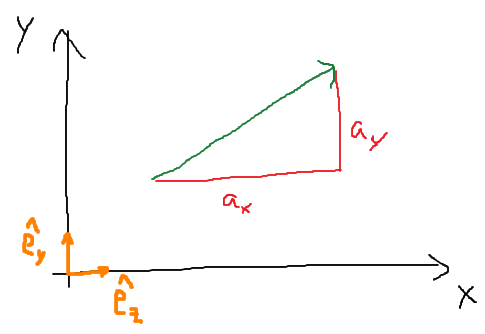
\includegraphics[width=8cm]{vektor-komponenten.png}
    \centering
    \caption{Komponenten eines Vektors}
\end{figure} 
Dabei fällt auf, dass nirgendwo ein Startpunkt des Vektors spezifiziert wird. Das liegt daran, das Vektoren keinen Startpunkt haben, sondern allgemein an beliebiger Stelle anfangen können. Oftmals bieten sich aber bestimmte  Startpunkte zeichen- und rechentechnisch an. 

\section{Polarform von Vektoren}
Im Abschnitt Definition haben wir unseren Vektor entlang fest bestimmter Achsen zerlegt, das Koordinatensystem können wir aber beliebig legen und drehen, solange wir dabei die Komponenten neu bestimmen. Oftmals haben wir Situationen, in denen z.B. mehrere Kräfte wirken (kleiner Vorgriff). Dann müssen wir diese so zerlegen, dass die einzelnen Komponenten möglichst mit den Achsen zusammenfallen. \\

Oftmals kennen wir nur Länge $r$ eines Vektors und den Winkel $\alpha$ zu einer bestimmten Oberfläche. In diesen Fällen suchen wir meist die Komponenten dieser Vektoren entlang dieser Oberfläche, dafür können wir Trigonomotrie verwenden (s. Abb. 2). Wenn wir in Komponenten zerlegen, müssen wir darauf achten, dass diese senkrecht zueinander stehen, sonst sind sie nicht unabhängig und wir können sie außerdem nicht trigonometrisch bestimmen.
\begin{figure}[H]
    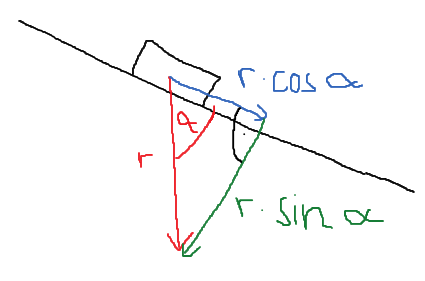
\includegraphics[width=8cm]{vektor-komponenten-trig.png}
    \centering
    \caption{Trigonometrische Bestimmung der Vektorkomponenten}
\end{figure}  
Wo zeigen die Einheitsvektoren bei dieser Zerlegung hin? \\

Diese Darstellungsart von Vektoren heißt Polarform, wir können zwischen Polarform und Komponentenform beliebig wechseln. Wie wir aus der Polarform die Kompoenenten finden, haben wir bereits herausgefunden, die Rückrichtung verläuft etwas anders. Die Länge eines Vektors berechnet sich aus den Komponenten zu: 
$$ r = \sqrt{r_x^2 + r_y^2} \text{ (nach Satz des Pythagoras)}$$
Den Winkel bestimmen wir zu: 
$$\alpha = \arctan\bigg(\frac{r_x}{r_y}\bigg)$$

\section{Grundrechenarten}
\textbf{Skalarmultiplikation} \\
Wenn wir einen Vektor mit einer "normalen Zahl", also einem Skalar multiplizieren, entspricht das einer Multiplikation der einzelnen Komponenten: 
$$c\vec{a} = \colvec{2}{ca_x}{ca_y}$$
Grafisch entspricht das einer Erhaltung der Richtung, aber einer ver-$c$-fachung der Länge. Für negative $c$ dreht sich die Richtung des Vektors um. \\\\
\textbf{Vektoraddition und -subtraktion} \\
Wenn wir zwei (oder mehr) Vektoren addieren/subtrahieren, addieren/subrahieren wir ihre Komponenten. Vektoraddition unterliegt dengleichen Rechenregeln wie die normale Addition. 
$$ \vec{a}+\vec{b} = \colvec{2}{a_x}{a_y}+\colvec{2}{b_x}{b_y} = \colvec{2}{a_x + b_x}{b_x+b_y}$$
$$ \vec{a}-\vec{b} = \colvec{2}{a_x}{a_y}+\colvec{2}{b_x}{b_y} = \colvec{2}{a_x - b_x}{b_x-b_y} $$
Dabei sind $a_x + b_x$ und $a_y + b_y$ die sogenannten \textbf{Komponentengleichungen}, diese werden uns noch öfter begegnen. 
Grafisch entspricht die Addition einem aneinanderlegen der Spitzen der Vektoren, bei der Subtraktion wird der Minuend davor umgedreht (Skalarmultiplikation mit $-1$): 
\begin{figure}[H]
    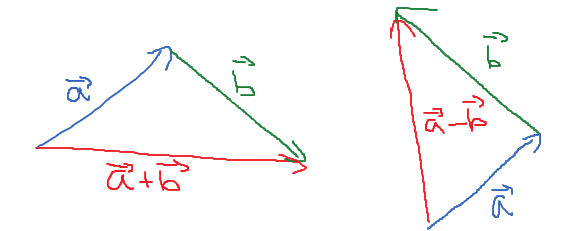
\includegraphics[width=8cm]{vektoraddition.png}
    \centering
    \caption{Trigonometrische Bestimmung der Vektorkomponenten}
\end{figure}  
\noindent Es gibt noch verschiedene andere Rechenarten, die aber bei der IJSO nicht hilfreich sind. 
\end{document}